\documentclass[tikz,border=2pt]{standalone}
\usepackage{amsmath,amssymb}
\usepackage{tikz}
\usetikzlibrary{arrows.meta}

\begin{document}
% The vocabulary by dimensions: n = 1 or n >= 2 inputs (univariate / multivariable) against
% k = 1 or k >= 2 outputs (real-valued / vector-valued), with a typical picture of each kind.
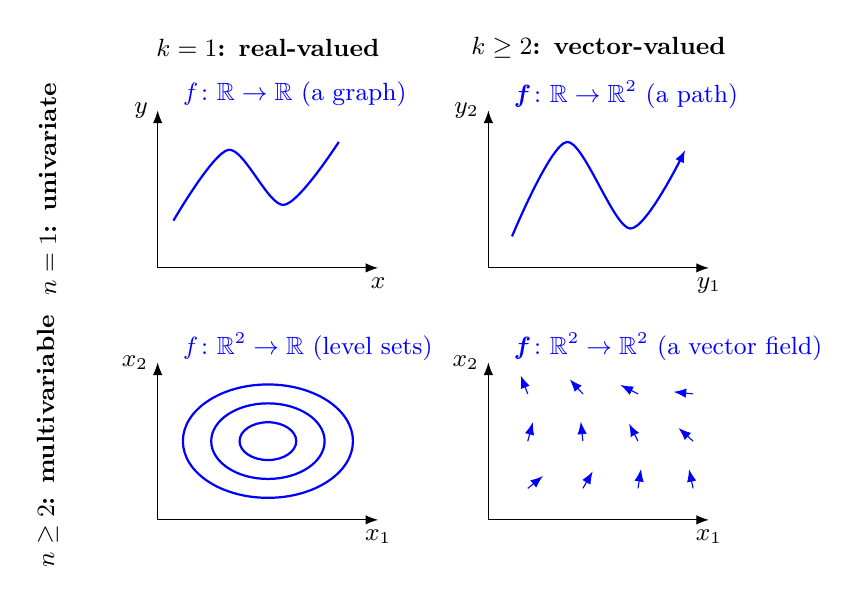
\begin{tikzpicture}[every node/.style={font=\small}, >={Latex[length=1.6mm]}]
	\node[font=\small\bfseries] at (2.2,3.1) {$k=1$: real-valued};
	\node[font=\small\bfseries] at (6.4,3.1) {$k\ge2$: vector-valued};
	\node[font=\small\bfseries, rotate=90] at (-0.6,1.3) {$n=1$: univariate};
	\node[font=\small\bfseries, rotate=90] at (-0.6,-1.9) {$n\ge2$: multivariable};
	\begin{scope}[shift={(0.8,0.3)}]
		\draw[->] (0,0) -- (2.8,0) node[below] {$x$};
		\draw[->] (0,0) -- (0,2) node[left] {$y$};
		\draw[blue, thick] plot[smooth] coordinates {(0.2,0.6) (0.9,1.5) (1.6,0.8) (2.3,1.6)};
		\node[blue, font=\small, anchor=west] at (0.2,2.2) {$f\colon\mathbb{R}\to\mathbb{R}$ (a graph)};
	\end{scope}
	\begin{scope}[shift={(5.0,0.3)}]
		\draw[->] (0,0) -- (2.8,0) node[below] {$y_1$};
		\draw[->] (0,0) -- (0,2) node[left] {$y_2$};
		\draw[blue, thick, ->] plot[smooth] coordinates {(0.3,0.4) (1.0,1.6) (1.8,0.5) (2.5,1.5)};
		\node[blue, font=\small, anchor=west] at (0.2,2.2) {$\boldsymbol{f}\colon\mathbb{R}\to\mathbb{R}^2$ (a path)};
	\end{scope}
	\begin{scope}[shift={(0.8,-2.9)}]
		\draw[->] (0,0) -- (2.8,0) node[below] {$x_1$};
		\draw[->] (0,0) -- (0,2) node[left] {$x_2$};
		\foreach \r in {0.3,0.6,0.9} {\draw[blue, thick] (1.4,1) ellipse ({\r*1.2} and {\r*0.8});}
		\node[blue, font=\small, anchor=west] at (0.2,2.2) {$f\colon\mathbb{R}^2\to\mathbb{R}$ (level sets)};
	\end{scope}
	\begin{scope}[shift={(5.0,-2.9)}]
		\draw[->] (0,0) -- (2.8,0) node[below] {$x_1$};
		\draw[->] (0,0) -- (0,2) node[left] {$x_2$};
		\foreach \x in {0.5,1.2,1.9,2.6} {\foreach \y in {0.4,1.0,1.6} {
			\draw[blue, ->] (\x,\y) -- ({\x+0.25*cos(60*\y+30*\x)},{\y+0.25*sin(60*\y+30*\x)});
		}}
		\node[blue, font=\small, anchor=west] at (0.2,2.2) {$\boldsymbol{f}\colon\mathbb{R}^2\to\mathbb{R}^2$ (a vector field)};
	\end{scope}
\end{tikzpicture}
\end{document}
